\section{确界的概念和确界存在定理}
 \subsection{练习题}
     \begin{exercise}
         试证明确界的唯一性.
     \end{exercise}
     \begin{solution}
         反证.不妨设有$a>b$都为$A$上确界,

         取$0<\varepsilon<a-b$,则由确界定义知$\exists\, a_n>a-\varepsilon>b$且$a_n<a$;这与$b$也为上确界矛盾,故上确界唯一.下确界同理可证.
     \end{solution}

     \begin{exercise}
         设对每个$x\in A$成立$x<a$.问:在$\sup A<a$和$\sup A\leqslant a$中哪个是对的?
     \end{exercise}

     \begin{solution}
         后者.显然$\sup A\leqslant a$必然成立.

         设$A=\left\{1-(\frac{1}{2})^n\,\bigg\lvert\,n\in N_+\right\}$,显然$x<1$对$x\in A$都成立,而无论多小的$\varepsilon$,都$\exists\,n\in N_+\,s.t.\,1-(\frac{1}{2})^n>1-\varepsilon$,即$\sup A=1$.
     \end{solution}

     \begin{exercise}
         设数集$A$以$\beta$为上界,又有数列$\{x_n\}\subset A$和$\lim_{n\to\infty}x_n=\beta.$证明$\beta=\sup A$.
     \end{exercise}

     \begin{solution}
         由收敛定义可知无论多小的$\varepsilon>0$都$\exists\,N\in N_+\,s.t.\,n>N,\beta-x_n<\varepsilon\Rightarrow\beta-\varepsilon<x_n$.这就是上确界定义.
     \end{solution}

     \begin{wrapfigure}{r}{3.5cm}
         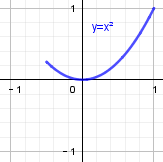
\includegraphics[width=3.5cm]{Picture/3.1/图一.png}
         \caption{}
     \end{wrapfigure}
     \begin{exercise}
         求下列数集的上确界和下确界:
         \begin{enumerate}
             \item $\{x\in Q\,\lvert\, x>0\};$
                   \begin{solution}
                       显然下确界是0,上确界是$+\infty$.
                   \end{solution}
             \item $\{y\,\lvert\, y=x^2,x\in(-\frac{1}{2},1)\};$
                   \begin{solution}
                       如右图所示,下确界为0,上确界为1.
                   \end{solution}
             \item $\left\{\left(1+\frac{1}{n}\right)^n \,\bigg\lvert\, n\in N_+\right\};$
                   \begin{solution}
                       下确界为2,上确界为$e$.

                       前已证$\left(1+\frac{1}{n}\right)^n$单调递增且极限为$e$.
                   \end{solution}
             \item $\{ne^{-n}\,\lvert\, n\in N_+\};$
                   \begin{solution}
                       前后两项的比值为$\frac{1}{e}\cdot\frac{n+1}{n}<\frac{2}{e}<1$,故数列$\left\{\frac{n}{e^n}\right\}$单调递减.而且上一章已证$\left\{\frac{n^q}{p^n}\right\}\to 0(p>1)$,所以下确界为0,上确界为$\frac{1}{e}$.
                   \end{solution}
             \item $\{\arctan x \,\lvert\, x\in (-\infty,+\infty)\};$
                   \begin{solution}
                       上下确界为$\pm \frac{\pi}{2}$.下证上确界.

                       由于$\arctan x$值域在$\left(-\frac{\pi}{2},\frac{\pi}{2}\right)$,而$\tan x$在此集合上单调增,故对任意小的$\varepsilon$,欲使$\arctan n>\frac{\pi}{2}-\varepsilon$,只需$\tan(\arctan n)=n>\tan\left(\frac{\pi}{2}-\varepsilon\right)$即可.

                   \end{solution}
             \item $\left\{(-1)^n+\frac{1}{n}(-1)^{n+1}\,\biggl\lvert\, n\in N_+\right\};$
                   \begin{solution}
                       上下确界为$\pm 1$.

                       从感性可以认知到集合中的数从中间向外边(-1和1)扩,对于任意小的$\varepsilon$,只需取$n$使$\frac{1}{n}<\varepsilon$即可.
                   \end{solution}
             \item $\left\{1+n\sin\frac{n\pi}{2}\,\bigg\lvert\, n\in N_+\right\}$.
                   \begin{solution}
                       上下确界为$\pm \infty$.

                       无论多大的M,都存在$n>M$且为$4k+1$(k为正整数)使$1+n\sin\frac{n\pi}{2}=1+n>M$;

                       同理也存在$n>-M-10$且为$4k+3$(k为正整数)使$1+n\sin\frac{n\pi}{2}=1-n<M$.
                   \end{solution}
         \end{enumerate}
     \end{exercise}

     \begin{exercise}
         证明:
         \begin{enumerate}
             \item $\sup\{x_n+y_n\}\leqslant \sup\{x_n\}+\sup\{y_n\}$;
                   \begin{solution}
                       因为对$n\in N_+$都成立$x_n+y_n<\sup\{x_n\}+\sup\{y_n\}$,故$\sup\{x_n\}+\sup\{y_n\}$也为$\{x_n+y_n\}$上界,而由上确界定义(上确界是所有上界中最小的一个)知命题成立.
                   \end{solution}
             \item $\inf\{x_n+y_n\}\geqslant\inf\{x_n\}+\inf\{y_n\}$.
                   \begin{solution}
                       解法与上题类似
                   \end{solution}
         \end{enumerate}
     \end{exercise}

     \begin{exercise}
         设有两个数集$A$和$B$,且对数集$A$中的任何一个数$x$和数集$B$中的任何一个数$y$成立不等式$x\leqslant y$.证明:\,$\sup\{x_n\}\leqslant\{y_n\}$.
     \end{exercise}
     \begin{solution}
         由题知,$\{y_n\}$中元素全是$\{x_n\}$上界,而由定义知命题成立.
     \end{solution}

     \begin{exercise}
         设数集$A$有上界,数集$B=\{x+c\,\lvert\, x\in A\}$,其中$c$是一个常数.证明:\,
         \[
             \sup B=\sup A+c,\inf B=\inf A+c.
         \]
     \end{exercise}
     \begin{solution}
         只证上确界.

         显然$\sup B\leqslant\sup A+c$.由定义知无论多小的$\varepsilon$,都存在$n$使得$a_n>\sup A-\varepsilon$,即$a_n+c>\sup A+c-\varepsilon$,故$\sup B=\sup A+c$.下确界证法完全类似.
     \end{solution}

     \begin{exercise}
         设$A,B$是两个有上界的数集,又有数集$C\subset \{x+y\,\lvert\, x\in A,y\in B\}$,则$\sup C\leqslant \sup A+\sup B$.举出成立严格不等号的例子.
     \end{exercise}
     \begin{solution}
         挺显然的.

         因为由定义有$x<\sup A,y<\sup B$,即$\sup A+\sup B$是$\{x+y\,\lvert\,x\in A,y\in B\}$一个上界,

         故有$\sup \{x+y\,\lvert\,x\in A,y\in B\}\leqslant\sup A+\sup B$,而$C\subset \{x+y\,\lvert\,x\in A,y\in B\}$,

         所以$\sup C\leqslant \{x+y\,\lvert\,x\in A,y\in B\}\leqslant\sup A+\sup B$.

         例如$A=\{1,2\},B=\{2,3\};C=\{3\}$.
     \end{solution}

     \begin{exercise}
         设$A,B$是两个有上界的数集,又有数集$C\supset  \{x+y\,\lvert\, x\in A,y\in B\}$,则$\sup C\geqslant \sup A+\sup B$.举出成立严格不等号的例子.
     \end{exercise}
     \begin{solution}
         与上题完全类似.
     \end{solution}
     \begin{note}
         (合并以上两题可见:当且仅当$C=\{x+y\,\lvert\, x\in A,y\in B\}$时成立$\sup C=\sup A+\sup B$.)
     \end{note}
